\documentclass[10pt,a4paper, draft]{article}

\usepackage{graphicx}
\usepackage[left=2cm,right=2cm,top=2cm,bottom=2cm]{geometry}

\begin{document}

\section{Top Level Translation}
When translating an SCJ program it is useful to start at the top of the program hierarchy, at the Safelet, and work downwards, towards the schedulable objects. This methodology ensures that all the paradigm objects in the program are captured. We organise the model of an SCJ program in to several tiers, which each encapsulate several components. The Safelet Tier contains the program's safelet and any possible top-level mission sequencers. A Mission Tier contains several Clusters, each of which is a mission and its schedulable objects. In order to identify the paradigm objects we must apply various rules, we describe these below.

\subsection{Safelet Tier}

Identifying the Saflet is relatively simple because there is only one in the program. Therefore to capture the Safelet we simply find the class that implements \texttt{javax.safetycritical.Safelet}. To capture the top-level mission sequencers, we identify any class that implements \texttt{javax.safetycritical.MissionSequencer} and could be returned by the Safelet's  \texttt{getSequencer()} method. 

\subsection{Mission Tiers}

Each program will have at least one tier (because a program must have at least one mission and one schedulable object) so our model always has Mission~Tier~0 to represent this. There may be as many other Mission~Tiers as needed to model the program. Each tier is composed of at least one cluster, which is a mission and its associated schedulables.

To capture Mission~Tier~ 0 we find each mission that may be returned by a top~level sequencer and each schedulable that may be registered in a Tier~0 mission's \texttt{initialize()} method. These processes are organised into clusters of each mission with its associated schedulables. 

The existence of other tiers is indicated by a Tier 0 cluster that contains a nested mission sequencer as one of its schedulable objects. To capture Mission~Tier~1, for example, we find any missions that may be returned by the \texttt{getNextMission()} method of a Tier~0 mission sequencer and their associated schedulables, which are any schedulables that may be registered in the \texttt{initialize()} method of these missions. Again, these mission and their associated schedulables are organised into clusters.  

One thing to note is that the clusters from the same mission sequencer will execute sequentially, whereas clusters from different missions in the same tier will execute in parallel. 

\subsection{Example}

As an example of the way we identify the tiers within a program we consider the Aircraft mode change example. Figure~\ref{AircraftDiagram} shows the processes in our model of the program. 

\begin{figure}
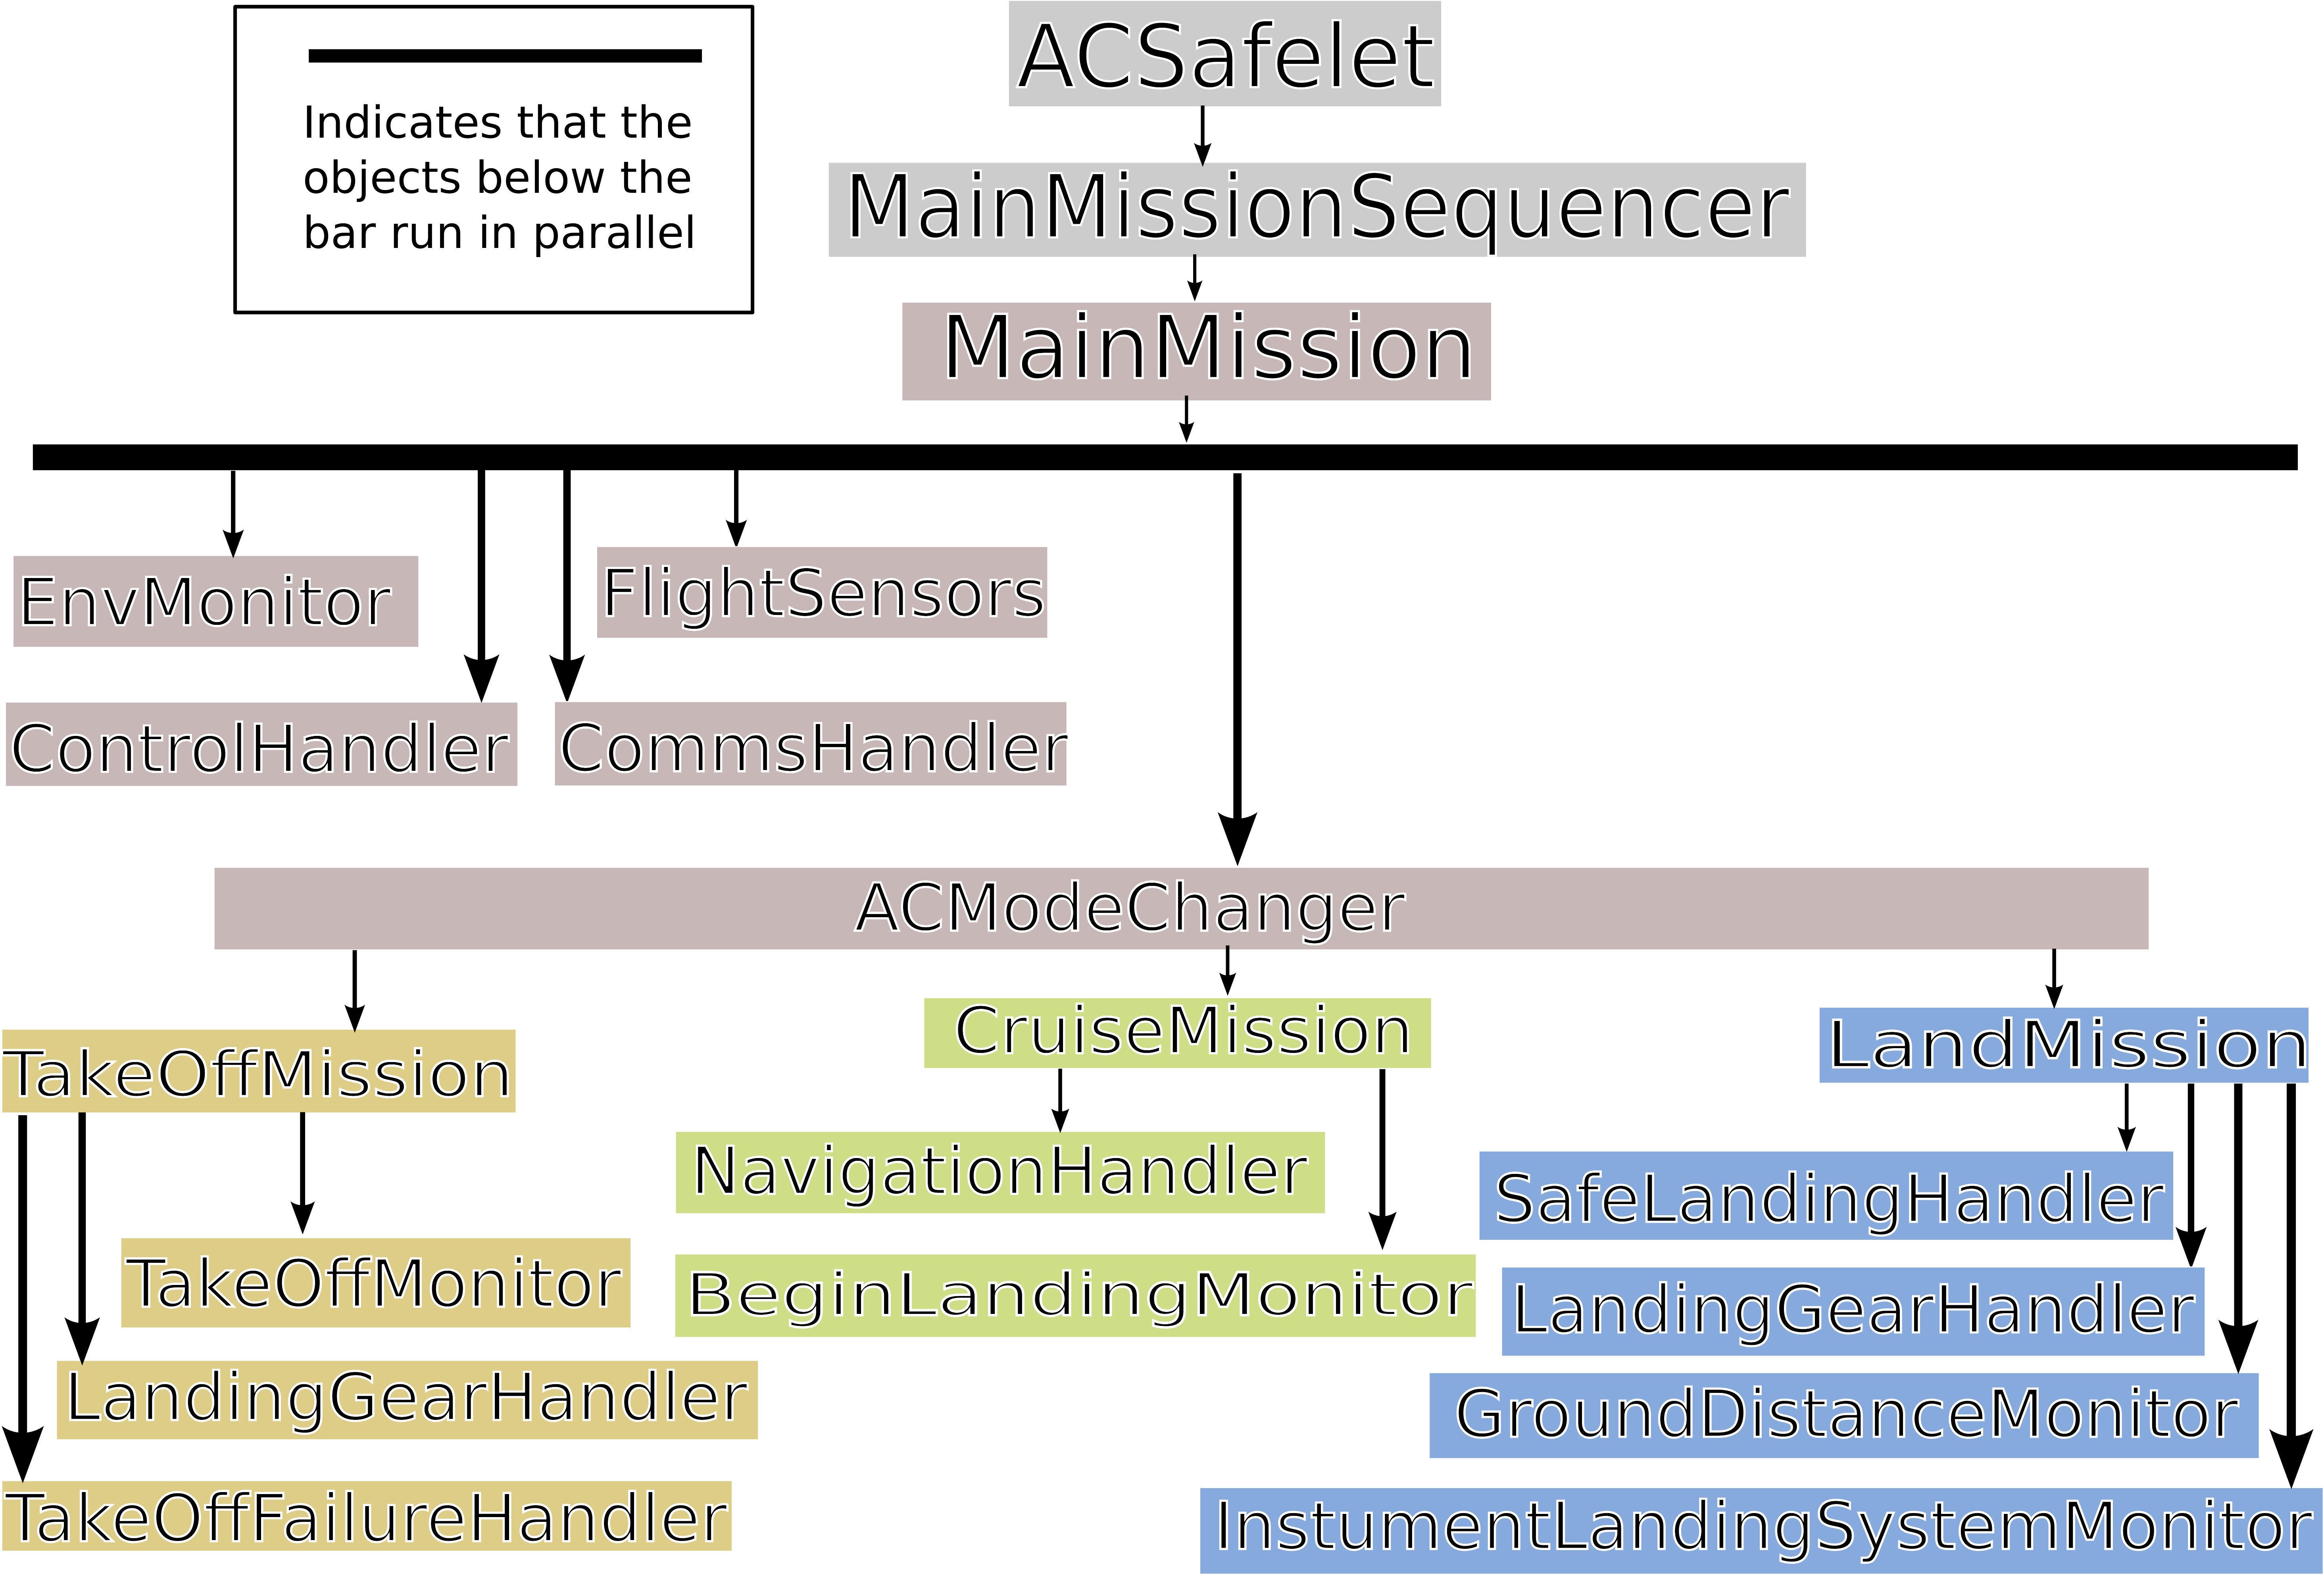
\includegraphics[width=\textwidth]{AircraftStructure.png}
\caption{The processes in the model of the Aircraft mode change application \label{AircraftDiagram}}
\end{figure}

The Safelet~Tier contains the $ACSafelet$ and $MainMissionSequencer$ processes. Mission~Tier~0 contains one cluster that pairs the $MainMission$ process with the processes modelling the four handlers ($EnvMoniotr$, $FlightSensors$, $ControlHandler$, $CommsHandler$) and the $ACModeChanger$ process, which is the nested mission sequencer . 

Mission~Tier~1 contains three clusters. Each cluster pairs a single mission with the schedulable objects that it may register. One cluster pairs the $TakeOffMission$ process with the processes $TakfeOffMonitor$, $LandingGearHandler$, and $TakeOffFailureHandler$. The second cluster pairs the $CruiseMission$ process with the $NavigationHandler$ and $BeginLandingMonitor$ processes. The final cluster pairs the $LandMission$ process with the $SafeLandingHandler$, $LandingGearHandler$, $GroundDistanceMonitor$, and $InstrumentLandingSystemMonitor$ processes. 


\end{document}